\chapter{IaaS and PaaS bootstrapping}\label{iaas-and-paas-bootstrapping}

This chapter describes how to bootstrap the IaaS and PaaS on top of it,
in order to deploy a cluster built around CoreOS, Kubernetes and
OpenShift. There is the need of compute, network and storage, in general
of an Infrastructure on top of which running these hosts. It's needed a
public cloud provider and a provisioning tool.

\begin{figure}[htbp]
\centering
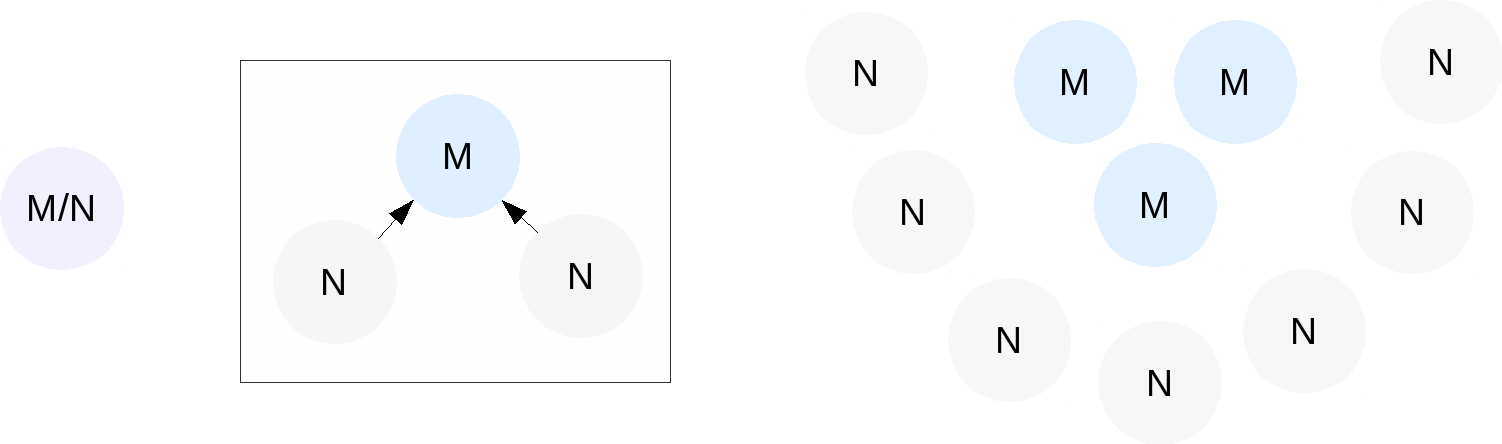
\includegraphics{media/ch4-clusters.png}
\caption{Cluster variants}
\end{figure}

\section{IaaS Providers}\label{iaas-providers}

In order to avoid too provider lock-in, will be used only
infrastructure-level services.

There is needed of a Public Cloud Provider with the following features:

\begin{itemize}
\itemsep1pt\parskip0pt\parsep0pt
\item
  CoreOS native support or possibly to make custom images
\item
  integration with existing tools (Terraform in particular)
\end{itemize}

Optionally:

\begin{itemize}
\itemsep1pt\parskip0pt\parsep0pt
\item
  DNS management
\item
  private network
\item
  based on free software
\item
  simple plans
\item
  possibly economic, no charge for intra-cluster traffic
\end{itemize}

Unfortunately RackSpace is the unique service built on top of OpenStack,
a free software solution. Anyway, the choice is \emph{Digital Ocean} who
match several points, providing however a KVM/QEMU-based public cloud.

\section{Provisioning of IaaS}\label{provisioning-of-iaas}

In addition, there is the need of automate the provisioning of the
infrastructure, and there are several tools.

\emph{Ansible} and \emph{SaltStack} are popular choices today and
includes modules for cloud provisioning, application deployment and
configuration management. Since the application and configuration part
is managed by OpenShift, theese tools are oversized.

\emph{Terraform} is a lot more minimal, focuses only on cloud
infrastructure provisioning, and it's more powerful because mantain the
state of infrastructure. So at every operation, Terraform generate the
difference between actual state (with multiple storage backends support)
and the desired state of users, and apply the necessary operations. For
example, Terraform enables powerful features like horizontal host-level
autoscaling varying the cardinality of cluster in response to global
load changes.

Terraform make possible applying the so called \emph{Infrastructure as
Code} (IaC), consist in versioning the project, so it tracks the
infrastructure evolution, such as in software development. This
represents a more structured, deterministic and reproducible way to
infrastructure management.

Terraform (https://terraform.io/) has to:

\begin{itemize}
\itemsep1pt\parskip0pt\parsep0pt
\item
  resolve the dependencies graph of infrastructure resources
\item
  connect to the cloud provider via REST APIs
\item
  upload the public SSH key used for host connection
\item
  provisioning the VMs in a specific data center with specific version
  of CoreOS
\item
  setting up the DNS in order to point to a node of the cluster
\item
  bootstrapping the hosts via SSH
\end{itemize}

\begin{figure}[htbp]
\centering
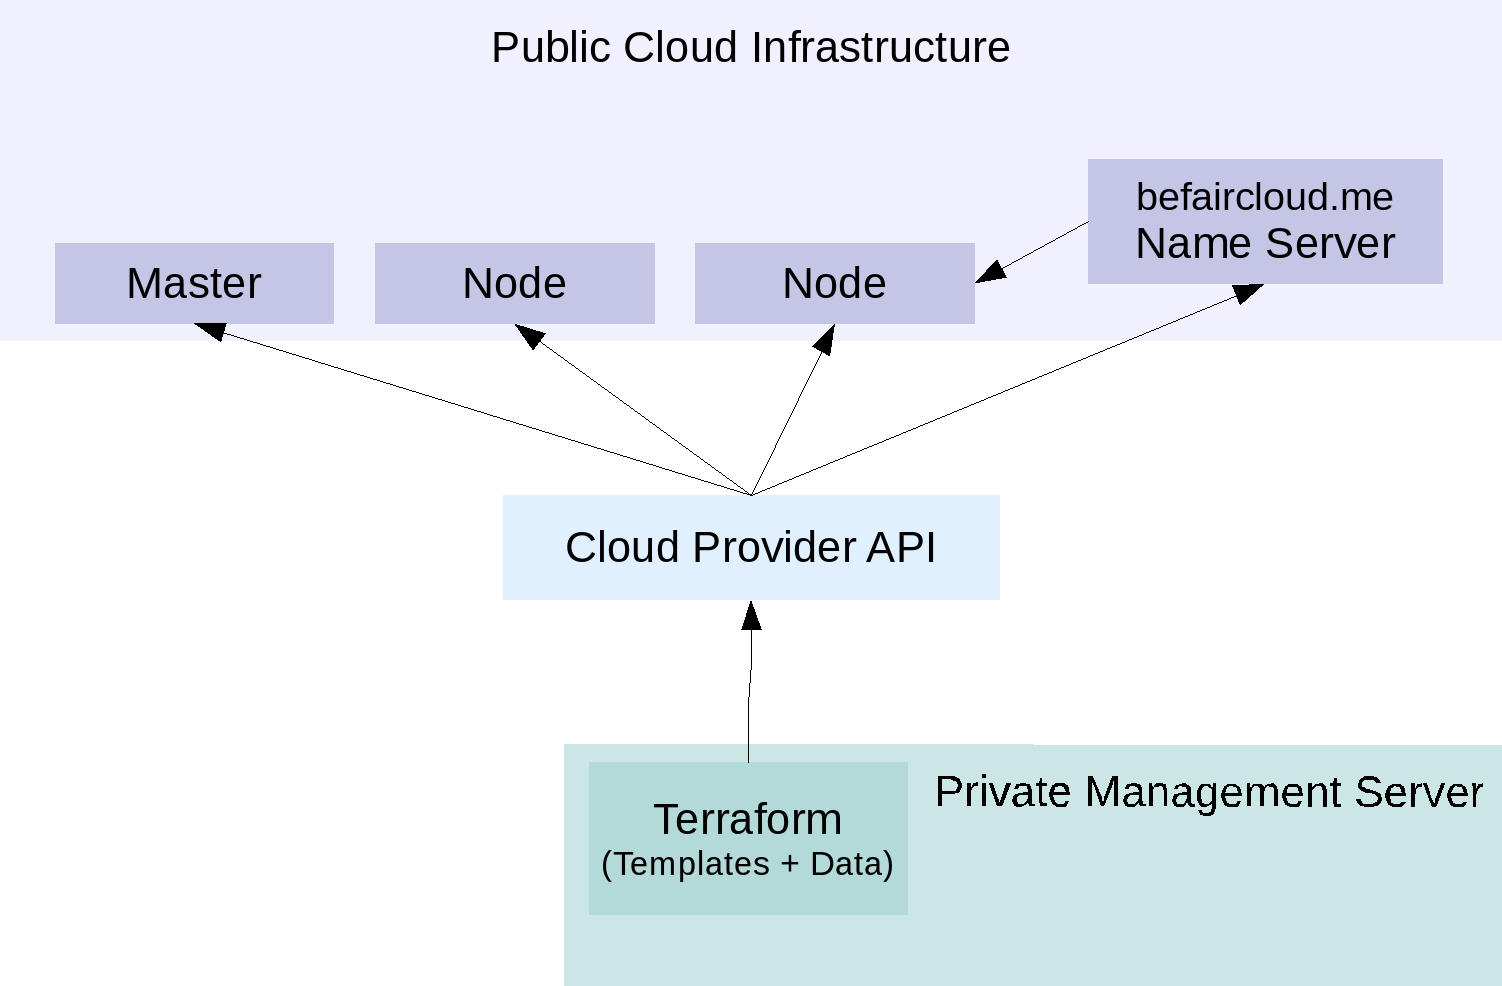
\includegraphics{media/ch4-terraform.png}
\caption{Infrastructure Provisioning with Terraform}
\end{figure}

\begin{figure}[htbp]
\centering
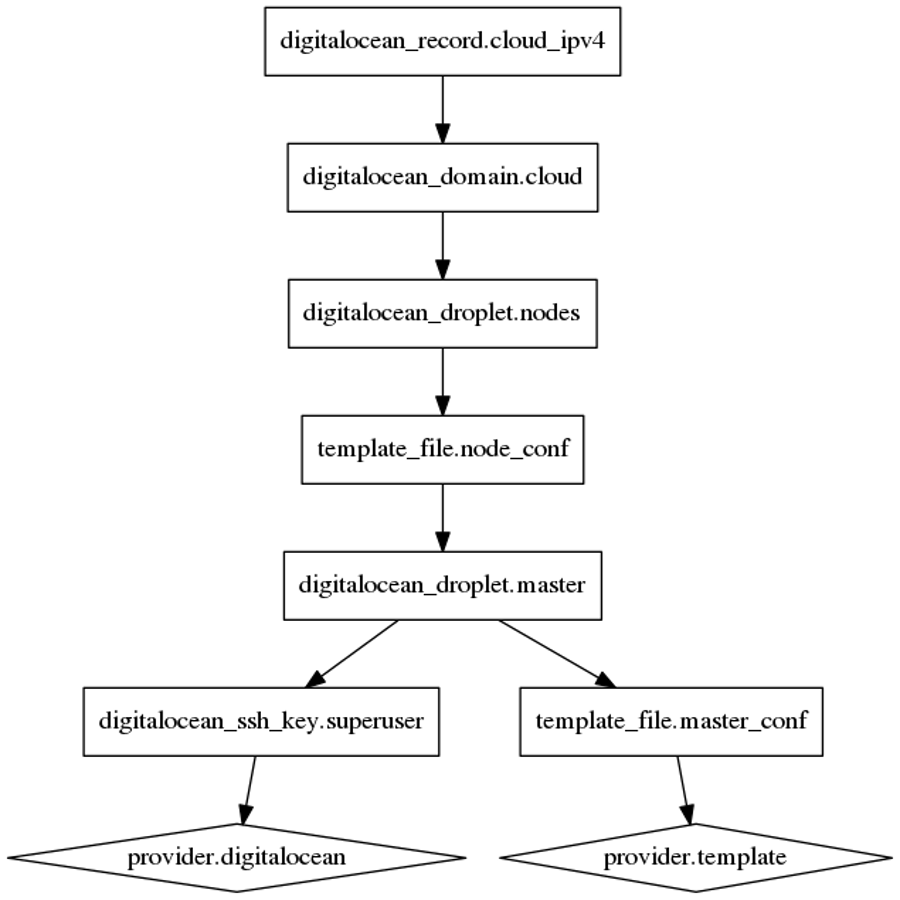
\includegraphics{media/ch4-graph.png}
\caption{Infrastructure Dependency Graph}
\end{figure}

Terraform supports JSON and a custom language for configuration, the
\emph{Hascicorp Configuration Language} (HCL). While it's a TOML-like
language, it remains a new language to learn, so the choice is to use a
human-readable and clean YAML, then automatically compile to JSON.

In terraform there are \emph{variables} for parametrization:

In order to connect to \emph{provider} API, there is the need of an
access token (generated from the Digital Ocean Web UI):

Then, there are all managed \emph{resources}, that can be splitted in
\emph{templates}:

The \emph{SSH public key} for access to hosts:

The \emph{virtual machines} of master and nodes:

Since there is a dedicated domain for this project, it will be managed
the Digital Ocean DNS service in order to point \emph{befaircloud.me}
domain to the first node where there is \emph{HAProxy} for external
routing:

At the end, there is some output with commands for complete the
bootstrapping and log via SSH to master.

\begin{verbatim}
Outputs:

  step1 = scp -r -i .cache/id -o StrictHostKeyChecking=no core@46.101.133.104:./master .cache/; \
scp -r -i .cache/id -o StrictHostKeyChecking=no .cache/master core@46.101.138.191:./; \
scp -r -i .cache/id -o StrictHostKeyChecking=no .cache/master core@46.101.200.100:./

  step2 = log to master -- ssh -i .cache/id -o StrictHostKeyChecking=no core@46.101.133.104
log to node-0 -- ssh -i .cache/id -o StrictHostKeyChecking=no core@46.101.138.191
log to node-1 -- ssh -i .cache/id -o StrictHostKeyChecking=no core@46.101.200.100
dashboard -- https://46.101.133.104:8443
entrypoint -- http://befaircloud.me
\end{verbatim}

\section{Provisioning of PaaS}\label{provisioning-of-paas}

IaaS provides servers starting from vanilla CoreOS image, so it needed
provide some configuration for PaaS bootstrapping. For this purpose has
been used \emph{Cloud Config}, an emerging standard for operating system
configuration at boot time via a declarative way.

Cloud Config consists of a simple YAML file with \emph{hostname},
\emph{ssh\_authorized\_keys}, \emph{write\_files} and other values.
CoreOS added some custom value for cluster upgrade mode, configurations
of SystemD units.

Since master and node have a different configuration needs, there are
been developed two templates. Terraform use these templates and passing
them when requesting the machines. The main dependency is provide the
master private IPv4 address to nodes, so they can connect to the master.

Thanks to this capacilities, this process is quite totally automated
except for a single command, that is anyway automatically provided by
Terraform at the end of boostrapping process.

\begin{figure}[htbp]
\centering
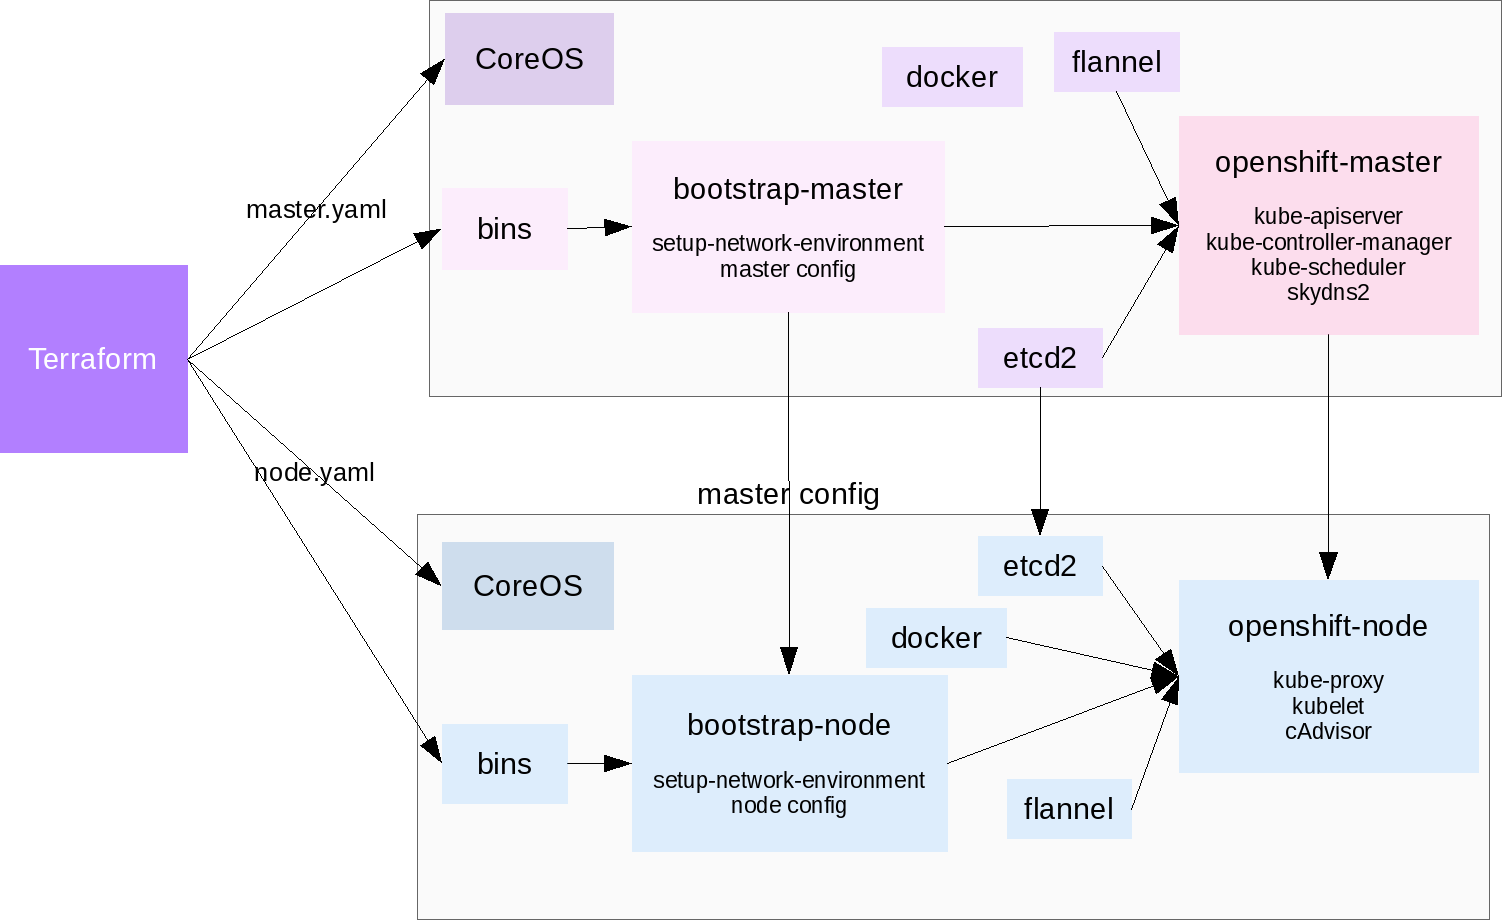
\includegraphics{media/ch4-bootstrap.png}
\caption{Provisioning of the PaaS}
\end{figure}